\section{Обзор предметной области}
\label{sec:domain}
В данном разделе будет произведён обзор предметной области задачи, решаемой в рамках дипломного проекта;
% рассмотрены вопросы о сущности байесовых сетей и принципе их работы; приведена оценка сложности различных проблем, возникающих при применении вероятностных сетей для решения прикладных задач.
% Также будут рассмотрены принципы работы алгоритмов вывода структуры по данным, реализованных в программном обеспечении разработанном в рамках дипломного проекта, и произведено сравнение с существующим ПО для решения схожих задач.

\subsection{Оперативные запоминающие устройства}
\label{sub:domain:ram}
Компактная микроэлектронная память находит широкое применение в самых различных по назначению электронных устройствах. Понятие «память» связывается с ЭВМ и определяется как ее функциональцая часть, предназначенная для записи, хранения и выдачи данных. Комплекс технических средств, реализующих функцию памяти, называется запоминающим устройством (ЗУ).

Микросхема памяти содержит выполненные в одном полупроводниковом кристалле матрицу-накопитель, представляющую собой совокупность элементов памяти (ЭП) и функциональные узлы, необходимые для управления матрицей-накопителем, усиления сигналов при записи и считывании, обеспечения режима синхронизации. Элемент памяти может хранить один разряд числа, т. е. один бит информации.

По назначению микросхемы памяти делят на две группы: для оперативных запоминающих устройств (ОЗУ) и для постоянных запоминающих устройств (ПЗУ). ОЗУ предназначено для использования в условиях, когда необходимо выбирать и обновлять хранимую информацию. Вследствие этого в ОЗУ предусматриваются три режима работы: режим хранения при отсутствии обращения к ЗУ, режим чтения информации и режим записи новой информации. При этом в режимах чтения и записи ОЗУ должно функционировать с высоким быстродействием (время чтения или записи составляет доли микросекунды). В цифровых вычислительных устройствах ОЗУ используются для хранения промежуточных и конечных результатов обработки данных. При отключении источника питания информация в ОЗУ теряется. В условном графическом обозначении функция ОЗУ задается комбинацией символов «RAM» – random access memory (память с произвольным доступом) \cite{dram_tutorial}.

Существует два типа ОЗУ: статическое и динамическое. Статическое ОЗУ (Static RAM, SRAM) конструируется с использованием D-триггеров. Информация в ОЗУ сохраняется на протяжении всего времени, пока к нему подаётся питание: секунды, минуты, часы и даже дни. Статическое ОЗУ работает очень быстро. Обычно время доступа составляет несколько наносекунд. По этой причине статическое ОЗУ часто используют в качестве кэш-памяти второго уровня \cite{dram_tutorial2}.

В динамическом ОЗУ (Dynamic RAM, DRAM), напротив, триггеры не используются. Динамическое ОЗУ представляет собой массив ячеек, каждая из которых содержит транзистор и крошечный конденсатор. Конденсаторы могут быть заряженными и разряженными, что позволяет хранить нули и единицы. Поскольку электрический  заряд имеет тенденцию исчезать, каждый бит в динамическом ОЗУ должен обновляться(перезаряжаться) каждые несколько миллисекунд, чтобы предотвратить утечку данных. Поскольку об обновлении должна заботиться внешняя логика, динамическое ОЗУ требует более сложного сопряжения, чем статическое, хотя этот недостаток компенсируется большим объёмом \cite{dram_tutorial3}.

Поскольку динамическому ОЗУ нужен только один транзистор и один конденсатор на бит (статическому ОЗУ требуется в лучшем случае 6 транзисторов на бит), динамическое ОЗУ имеет очень высокую плотность записи (много битов на одну микросхему). По этой причине основная память почти всегда строится на основе динамических ОЗУ. Однако динамические ОЗУ работают очень медленно (время доступа занимает десятки наносекунд). Таким образом, сочетание кэш-памяти на основе статического ОЗУ и основной памяти на основе динамического ОЗУ соединяет в себе преимущества обоих устройств.

Существует несколько типов динамических ОЗУ. Самый древний тип, который все еще используется, - FPM (Fast sub Mode - быстрый постраничный режим). Это ОЗУ представляет собой матрицу битов. Аппаратное обеспечение представляет адрес строки, а затем - адреса столбцов. Благодаря явно передаваемым сигналам память работает асинхронно по отношению к главному тактовому генератору системы \cite{dram_book}.

FPM постепенно замещается памятью EDO (Extended Data Output - память с расширенными возможностями вывода), которая позволяет обращаться к памяти еще до того, как закончилось предыдущее обращение. Такой конвейерный режим, хотя и не ускоряет доступ к памяти, повышает пропускную способность, позволяя получить больше слов в секунду.

Память типа FPM и EDO сохраняла актуальность в те времена, когда продолжительность цикла работы микросхем памяти не превышала 12 нс. Впоследствии, с увеличением быстродействия процессоров, сформировалась потребность в более быстрых микросхемах памяти, и тогда на смену асинхронным режимам FPM и EDO пришли синхронные динамические ОЗУ (Synchronous DRAM, SDRAM). Синхронное динамическое ОЗУ управляется от главного системного тактового генератора. Данное устройство представляет собой гибрид статического и динамического ОЗУ. Основное преимущество синхронного динамического ОЗУ состоит в том, что оно исключает зависимость микросхемы памяти от управляющих сигналов. ЦП сообщает памяти, сколько циклов следует выполнить, а затем запускает её. Каждый цикл на выходе дает 4, 8 или 16 бит в зависимости от количества выходных строк. Устранение зависимости от управляющих сигналов приводит к ускорению передачи данных между ЦП и памятью \cite{ibm_dram_article}.

Следующим этапом в развитии памяти SDRAM стала память DDR (Double Date Rate - передача данных с двойной скоростью). Эта технология предусматривает вывод данных как на фронте, так и на спаде импульса, вследствие чего скорость передачи увеличивается вдвое. Например, 8-разрядная микросхема такого типа, работающая с частотой 200 МГц, дает на выходе два 8-разрядных значения 200 миллионов раз в секунду (разумеется, такая скорость удерживается в течение небольшого периода времени); таким образом, теоретически, кратковременная скорость может достигать 3,2 Гбайт/с. Интерфейсы памяти DDR2 и DDR3 обеспечивают дополнительный прирост производительности по сравнению с DDR за счет повышения скорости шины памяти до 533 МГц и 1067 МГц соответственно.

\subsubsection{Динамические оперативные запоминающие устройства}
\label{sub:domain:ram:dram}
Как уже отмечалось, информация в ячейке динамического ОЗУ представлена в виде наличия или отсутствия заряда на конденсаторе. Схема ячейки памяти ЯП динамического ЗУ на одном МОП–транзисторе с индуцируемым p-каналом представлена на рисунке~\ref{fig:domain:ram:dram:dram_cell} (выделена пунктирной линией). На схеме также показаны общие элементы для n-ячеек одного столбца. Главное достоинство этой схемы - малая занимаемая площадь. Накопительный конденсатор C1 имеет МДП-структуру и изготавливается в едином технологическом цикле. Величина его емкости составляет сотые доли пикоФарад. Конденсатор C1 хранит информационный заряд. Транзистор VT1 выполняет роль переключателя, передающего заряд конденсатора в разрядную шину данных ШД при считывании, либо заряжающего конденсатор при записи. В режиме хранения на адресной линии A1 должен присутствовать потенциал логической единицы, под действием которого транзистор VT1 будет закрыт и конденсатор C1 отключен от шины данных ШД. Включение конденсатора в шину данных осуществляется логическим нулем на линии. При этом на транзистор VT1 подается напряжение, что приводит к его открыванию \cite{ibm_dram_article}.

\begin{figure}[ht]
\centering
  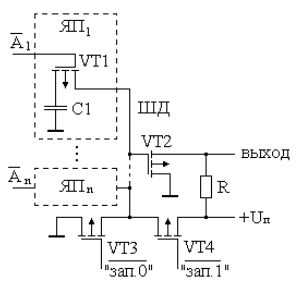
\includegraphics[scale=1]{a_dram_cell.png}  
  \caption{Принципиальная схема ячейки динамического ОЗУ}
  \label{fig:domain:ram:dram:dram_cell}
\end{figure}

Поскольку шина данных ШД объединяет все ячейки памяти данного столбца, то она характеризуется большой длиной и ее собственная емкость имеет существенное значение. Поэтому при открывании транзистора VT1 потенциал шины данных изменяется незначительно. Чтобы установившийся потенциал на ШД однозначно идентифицировать с уровнем напряжения логического нуля или логической единицы, используется усилитель на базе транзистора VT2 и резистора R. Непосредственно перед считыванием емкость шины данных подзаряжают подключением ее к источнику питания через транзистор VT4. Делается это для фиксации потенциала шины данных. При считывании информации происходит перераспределение заряда конденсатора и заряда шины данных, в результате чего информация, хранимая на конденсаторе С1, разрушается. Поэтому в цикле считывания необходимо произвести восстановление (регенерацию) заряда конденсатора. Для этих целей, а также для записи в ячейку памяти новых значений, используются транзисторы VT3 и VT4, которые подключают шину данных либо к источнику питания, либо к нулевому общему потенциалу. Для записи в ячейку памяти логической единицы необходимо открыть транзистор VT4 нулевым значением управляющего сигнала <</зап.1>> и подключить к шине данных источник питания. Для записи логического нуля необходимо нулевым потенциалом на входе «/зап.0» открыть транзистор VT3. Одновременная подача логических нулей на входы <</зап.1>>  и <</зап.0>> не допускается, так как это вызовет короткое замыкание источника питания на общий провод заземления.

На рисунке~\ref{fig:domain:ram:dram:dram_structure} показан пример структуры микросхемы динамического ОЗУ емкостью 64кбит. Данные в этой микросхеме памяти представлены как 64к отдельных бит, т.е. формат памяти 64к x 1. Ввод и вывод осуществляется раздельно, для чего предусмотрена пара выводов DI (вход) и DО (выход). Для ввода адреса имеется восемь контактов $A_0 - A_7$. Адресация к 64к ячейкам памяти осуществляется шестнадцатиразрядными адресами $A_0 - A_15$. Причем сначала на входы $A_0 - A_7$ подаются восемь младших разрядов $A_0 - A_7$ адреса, а затем – восемь старших разрядов $A_8 - A_15$. Восемь младших разрядов адреса фиксируются в регистре адреса строки подачей сигнала /RAS (сигнал выборки строки). Восемь старших разрядов адреса фиксируются в регистре адреса столбца подачей сигнала /CAS (сигнал выборки столбца). Такой режим передачи кода адреса называется мультиплексированным по времени. Мультиплексирование позволяет сократить количество выводов микросхемы. Ячейки памяти расположены в виде матрицы из 128 строк и 512 столбцов. Дешифратором строк вырабатывается адресный сигнал выборки $A_i$ ячеек памяти i-ой строки, т.е. выбирается одна из 128 строк. Обращение к строке вызывает подключение 512 ячеек памяти через соответствующие разрядные шины данных ШД этой строки к усилителям считывания (по одному на столбец). При этом автоматически происходит подзаряд запоминающих конденсаторов всех ячеек памяти выбранной строки до исходного уровня за счет передачи усиленного сигнала по цепи обратной связи. Этот процесс называется регенерацией памяти. Дешифратор столбцов выбирает один из 512 усилителей считывания. Бит, выбранный в режиме считывания, выдается на линию DО. Если одновременно с сигналом /CAS при предварительно установленном сигнале /RAS действует сигнал записи /WR, то бит с входа DI будет записан в выбранную ячейку памяти, при этом выход DО микросхемы остается в отключенном состоянии в течение всего цикла записи \cite{dram_tutorial}.

\begin{figure}[ht]
\centering
  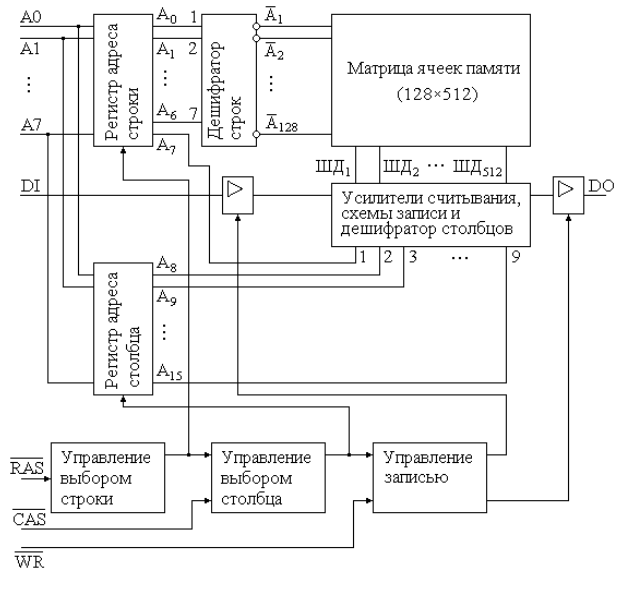
\includegraphics[scale=0.75]{a_dram_structure.png}  
  \caption{Принципиальная схема ячейки динамического ОЗУ}
  \label{fig:domain:ram:dram:dram_structure}
\end{figure}

На рисунке~\ref{fig:domain:ram:dram:dram_timing} представлены временные диаграммы, поясняющие работу динамического ОЗУ. В режиме считывания (рисунок~\ref{fig:domain:ram:dram:dram_timing},a) на адресные входы микросхемы подаются восемь младших разрядов $A_0 - A_7$ адреса, после чего вырабатывается сигнал /RAS, при этом производится выбор строки матрицы в соответствии с поступившим адресом. У всех ячеек памяти выбранной строки регенерируется заряд конденсаторов. Далее производится подача на адресные входы микросхемы восьми старших разрядов адреса, после чего вырабатывается сигнал /CAS. Этим сигналом выбирается нужная ячейка памяти из выбранной строки и считанный бит информации поступает на выход микросхемы DО. В режиме считывания промежуток времени между подачей сигнала /RAS и появлением данных на выходе DО называется временем выборки tв.

\begin{figure}[ht]
\centering
  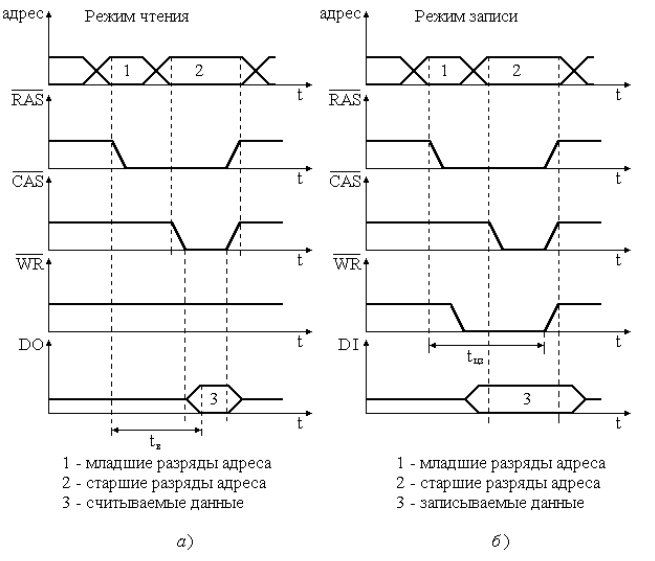
\includegraphics[scale=0.75]{a_dram_timing.png}  
  \caption{Временная диаграмма работы ОЗУ динамического типа}
  \label{fig:domain:ram:dram:dram_timing}
\end{figure}

В режиме записи (рисунок~\ref{fig:domain:ram:dram:dram_timing},б) за время цикла записи tцз принимается интервал времени между появлением сигнала /RAS и окончанием сигнала /WR. В момент появления сигнала /CAS записываемые данные уже должны поступать на вход DI. Сигнал /WR обычно вырабатывается раньше сигнала /CAS.

Для каждого типа микросхем динамических ОЗУ в справочниках приводятся временные параметры, регламентирующие длительность управляющих сигналов, подаваемых на микросхему, а также порядок их взаимного следования.
Заряд конденсатора динамического ОЗУ со временем уменьшается вследствие утечки, поэтому для сохранения содержимого памяти процесс регенерации каждой ячейки памяти должен производится через определенное время. Следовательно, для предотвращения разряда запоминающих конденсаторов необходимо обращаться к каждой строке матрицы через определенное время. При обычном режиме работы ОЗУ это условие не соблюдается, так как обращение к одним ячейкам происходит часто, а к другим очень редко. Поэтому необходим специальный блок, ответственный за регенерацию памяти. Этот блок должен при отсутствии обращений к ОЗУ со стороны внешних устройств циклически формировать на адресных входах $A_0 - A_6$ значения всех возможных адресов, сопровождая каждый из них управляющим сигналом /RAS, т.е. производить циклическое обращение ко всем 128 строкам матрицы ячеек памяти. Регенерацию необходимо проводить и в те моменты времени, когда ОЗУ используется устройствами, приостанавливая на время регенерации взаимодействие ОЗУ с этими устройствами, т.е. путем перевода этих устройств в режим ожидания.

Из изложенного выше следует, что использование динамического ОЗУ требует довольно сложной схемы управления. Если учесть, что обращение к ОЗУ со стороны устройств, с которыми оно работает, и обращение со стороны схемы регенерации не зависят друг от друга, следовательно, могут возникать одновременно, то необходима схема, обеспечивающая упорядоченность этих обращений. Для этих целей существуют схемы, управляющие работой динамических ОЗУ. Это так называемые контроллеры динамического ОЗУ, реализованные на одном кристалле. Их использование позволяет значительно упростить построение памяти на динамических ОЗУ.

Лидером в производстве микросхем динамического ОЗУ на сегодняшний день является фирма Samsung. Емкость одной микросхемы DRAM достигает значения 128 Мбайт и более. Кроме того, этой фирмой предлагается ряд передовых идей по обеспечению наибольшего быстродействия. Например, операции чтения и записи выполняются дважды за один такт – по переднему и заднему фронтам тактового импульса. Фирмой Mitsubishi предложена концепция встраивания в микросхемы динамической памяти статической кэш-памяти небольшого объема (Cashed DRAM), в которой хранятся наиболее часто запрашиваемые данные.

\subsection{Функциональные модели неисправностей ДОЗУ}
\label{sub:domain:faults}
Причиной неисправного состояния ОЗУ является наличие физического или механического дефекта либо множества подобных дефектов, количество и многообразие которых практически неограниченно. В зависимости от технологических особенностей при производстве ОЗУ и внешних факторов при его эксплуатации могут появляться новые типы и разновидности дефектов. Определение факта возникновения дефекта и его классификация представляется весьма трудоёмкой и зачастую неразрешимой задачей. 

Функциональные неисправности ОЗУ подразделяются на два подмножества: неисправности матрицы запоминающих элементов и неисправности электронного обрамления. Второе подмножество включает неисправности дешифратора адреса и неисправности логики чтения/записи. Доминирующее значение имеют неисправности матрицы запоминающих элементов.

К неисправностям матрицы запоминающих элементов ОЗУ относят неисправности, в которых участвуют: одна ячейка ОЗУ; две ячейки ОЗУ; несколько ячеек ОЗУ, в общем случае более чем две. 

К неисправностям, затрагивающим одну ячейку ОЗУ, относят неисправности типа SAF и TF \cite{faults}.

\textit{Константные неисправности} (Stuck-At Faults - SAF). Неисправный ЗЭ ОЗУ постоянно находится в состоянии логического нуля(SAF0) или логической единицы (SAF1), независимо от операций, выполняемых с неисправным ЗЭ и другими ЗЭ ОЗУ. Как и для случая произвольной логики, различают однократные и многократные константные неисправности.

\textit{Переходные неисправности} (Transition Faults - TF). Подобные неисправности характеризуются невозможностью перехода состояния неисправного ЗЭ из 0 в 1 (TF1 $\uparrow$) или из 1 в 0 (TF $\downarrow$) при выполнении соответствующих операций записи. Данный тип неисправности достаточно близок по своей сути к константным неисправностям. Действительно, если ячейка, имеющая переходную неисправность, оказывается в состоянии, из которого она не может перейти в другое, ее поведение повторяет поведение ячейки, содержащей константную неисправность.

Среди неисправностей, в которых участвуют две ячейки ЗУ, выделяют неисправности типа CF и PSF.

\textit{Неисправности взаимного влияния} (Coupling Fault - CF). При описании данной неисправности выделяют влияющий ЗЭ (i - Aggressor Cell), изменение логического состояния которого воздействует на состояние зависимого ЗЭ (j - Victim Cell). Неисправности взаимного влияния CF подразделяются на три типа:
\begin{enumerate}
\item \textit{Инверсные неисправности взаимного влияния} (Inverse Coupling Faults - CFin). При наличии данной неисправности изменение значения bi влияющего ЗЭ вызывает инвертирование значения $b_j$ зависимого ЗЭ. Возможны следующие виды неисправностей CFin: $\wedge$($\uparrow$, $b_j$*), $\wedge$($\downarrow$, $b_j$*), $\vee$($\uparrow$, $b_j$*), $\vee$($\downarrow$, $b_j$*). Символ $\wedge$ и символ $\vee$ задают взаимное расположение влияющего и зависимого запоминающих элементов ОЗУ. Первый символ $\wedge$ означает, что ЗЭ с меньшим адресом влияет на ЗЭ с большим адресом (i<j), а символ $\vee$ используется в случае, когда адрес влияющего ЗЭ больше адреса зависимого ЗЭ (i>j).
\item \textit{Неисправности взаимного влияния прямого действия} (Idempotent Coupling Faults - CFid). При изменении значения bj влияющего ЗЭ происходит принудительная установка определённого логического значения 0 или 1 в зависимом ЗЭ. Различают восемь неисправностей прямого действия: $\wedge$($\uparrow$,0), $\wedge$($\uparrow$,1), $\wedge$($\downarrow$,0), $\wedge$($\downarrow$,1), $\vee$($\uparrow$,0), $\vee$($\uparrow$,1), $\vee$($\downarrow$,0) и $\vee$($\downarrow$,1). При исследовании эффективности тестов ОЗУ анализируется их покрывающая способность для всех 12 неисправностей взаимного влияния, в которых участвуют две ячейки (2-Coupling Faults) \cite{faults}.
\item \textit{Статические неисправности взаимного влияния} (State Coupling Faults -CFst). Переход зависимого ЗЭ в какое либо состояние $b_j$ возможен при определённом значении $b_i$ влияющего ЗЭ. Возможно восемь неисправностей CFst: $\wedge$(0,0), $\wedge$(0,1), $\wedge$(1,0), $\wedge$(1,1), $\vee$(0,0), $\vee$(0,1), $\vee$(1,0) и $\vee$(1,1).
\end{enumerate}

\textit{Кодочувствительные неисправности} (Pattern Sensitive Faults - PSF) рассматриваются как обобщение моделей неисправностей взаимного влияния. Для подобных неисправностей логическое состояние или изменение логического состояния одного ЗЭ ОЗУ может зависеть от содержимого (0 или 1) или от логических переходов из 1 в 0 или из 0 в 1 влияющих ЗЭ ОЗУ. В случае кодочувствительной неисправности PSF\textit{k}, в которой участвуют k запоминающих элементов ОЗУ, подразумевается, что влияющими ЗЭ в предельном случае могут быть любые \textit{k-1} из \textit{N} ЗЭ ОЗУ, а зависимым один из оставшихся \textit{N-k+1} ЗЭ. Такие неисправности называются неограниченными (Unrestricted) кодочувствительными неисправностями. Очевидно, что практическая значимость подобной модели невысока, так как сложность теста памяти и время его реализации при такой интерпретации кодочувствительной неисправности превышает всякие возможные пределы современных значений емкостей ЗУ. Поэтому при рассмотрении кодочувствительных неисправностей вводятся ограничения как на количество ЗЭ \textit{k}, так и на их местоположение \cite{faults}. 

При тестировании ОЗУ, как правило, придерживаются модели \textit{граничных кодочувствительных неисправностей} (Neighborhood Pattern Sensitive Faults - NPSF) как более реальной модели кодочувствительных неисправностей. Для таких моделей первым и необходимым ограничением является количество ЗЭ, участвующих в неисправности. Как правило, k не превышает 10, это следует из того факта, что для тестирования подобных неисправностей необходимо время пропорциональное величине $2^k$.
Вторым ограничением является физическое соседство ЗЭ. При этом зависимый ЗЭ называется \textit{базовым} ЗЭ (Base Cell), или базовой ячейкой, которая в данном случае является аналогом \textit{жертвы}, а остальные \textit{k-1} ЗЭ соседними ЗЭ (Neighborhood Cells), или \textit{соседними} ячейками, выступающими в роли агрессоров, количество и местоположение которых может быть произвольным. Поэтому на практике обычно используют модели кодочувствительных неисправностей NPSF\textit{k} с числом \textit{k}, равным 3, 5 и 9, конфигурации и обозначение которых приведены на рисунке~\ref{fig:domain:faults:neighbors}. 

\begin{figure}[ht]
\centering
  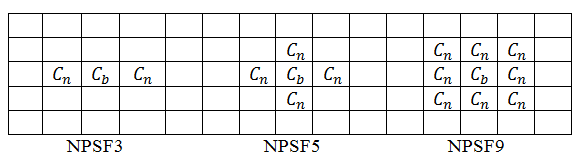
\includegraphics[scale=1]{a_faults_neighbors.png}  
  \caption{Модели кодочувствительных неисправностей}
  \label{fig:domain:faults:neighbors}
\end{figure}

Как видно из рисунка, в каждой из приведённых неисправностей в явном виде выделяется базовый ЗЭ - $C_b$ и соседние ЗЭ $C_n$, которые являются физическими соседями по отношению к базовому элементу.

В зависимости от эффекта влияния на базовый ЗЭ различают несколько классических типов кодочувствительных неисправностей NPSF\textit{k}.
\textit{Пассивными кодочувствительными неисправностями} (Passive NPSF - PNPSF) являются неисправности, при которых состояние базового ЗЭ не может быть изменено для определённого кода в \textit{k-1} соседних ЗЭ ОЗУ. 
\textit{Под активными кодочувствительными неисправностями} (Active NPSF - ANPSF) понимают неисправности, в которых базовый ЗЭ изменяет свое состояние из-за изменения кода в соседних ЗЭ. Изменение кода для подобных неисправностей происходит в результате изменения состояния на противоположное только в одном соседнем элементе, в то время как остальные ячейки сохраняют предыдущее состояние.
\textit{Статические кодочувствительные неисправности} (Static NPSF - SNPSF) характеризуются тем, что для определённой комбинации значений в соседних ЗЭ состояние базового ЗЭ принудительно устанавливается в состояние 0 или состояние 1. Главным отличием статических неисправностей от активных кодочувствительных неисправностей является длительность процесса установления неверного значения в базовой ячейке \cite{faults}.

Рассмотренные неисправности являются классическими и наиболее часто используются при тестировании ОЗУ. Однако существует и ряд других моделей неисправностей, также обсуждаемых и применяемых при тестировании памяти. В первую очередь здесь необходимо отметить \textit{неисправности дешифратора адреса} (Address Decoder Faults - AF), или \textit{адресные неисправности}. Однако обнаружение подобных неисправностей обеспечивается тестами, обнаруживающими неисправности матрицы ЗЭ.

Также к электронному обрамлению в большей мере относятся \textit{неисправности типа обрыв} (Stuck Open Fualt - SOF), которые также могут быть обнаружены при тестировании матрицы ОЗУ.
Логика чтение/запись обеспечивает интерфейс между массивом ячеек и внешней шиной данных. Данный функциональный блок может содержать те же типы неисправностей, что и массив ячеек памяти (SAF, TF, CFin, CFid). 
Модель типа \textit{разрушающая операция чтения} (Read Disturb Fault Model - RDF) практически аналогична неисправности \textit{слабый запоминающий элемент} (Weak Cell Fault Model - WCF) и обнаруживается путем внесения в классический маршевый тест временной задержки перед выполнением следующего маршевого элемента. Для ДОЗУ также характерна \textit{неисправность сохранения данных} (Data Retention Fault - DRF), которая, так же, как и неисправность RDF И WCF, обнаруживается путем внесения временных задержек в тест памяти.  

\subsection{Алгоритмы тестирования ДОЗУ}
\label{sub:domain:tests}
В условиях постоянного усложнения разрабатываемых средств электронной техники, как функционального, так и структурного (уже сегодня на подложке микропроцессора может быть расположено несколько миллионов транзисторов), в условиях необходимости быстрого продвижения уже разработанных устройств на рынок (быстрое моральное устаревание средств вычислительной техники) проблема надежного тестирования современных микропроцессоров и микропроцессорных систем становится все более актуальной. При этом очевидно, что качество и оперативность проектирования, эффективность и надежность функционирования микропроцессоров и микропроцессорных систем существенно зависят от качества и достоверности результатов решения задач их тестового диагностирования.

Рассмотрим классические методы тестирования ОЗУ.

\subsubsection{Тестирующий алгоритм Zero-One}
\label{sub:domain:tests:zero-one}
Тест Zero-One также известен как MSCAN. Он является достаточно простым и состоит из следующих шагов:
\begin{enumerate}
\item запись 0 во все ячейки памяти;
\item чтение ячеек памяти с ожидаемым значением 0;
\item запись 1 во все ячейки памяти;
\item чтение ячеек памяти с ожидаемым значением 1.
\end{enumerate}
Сложность данного теста составляет 4n. Не все неисправности типа Afs обнаруживаются. Неисправности типа SAFs обнаруживаются при условии исправного дешифратора адресов. Не все TFs и CFs обнаруживаются.

\subsubsection{Тестирующий алгоритм Checkboard}
\label{sub:domain:tests:checkboard}
Данный алгоритм предполагает создание сетки из нулей и единиц в шахматном порядке, как представлено на рисунке~\ref{fig:domain:tests:checkboard}. 

\begin{figure}[ht]
\centering
  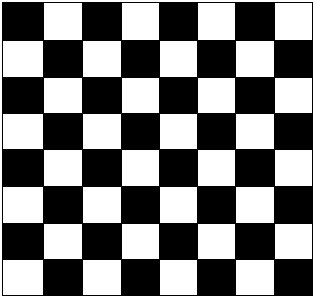
\includegraphics[scale=0.5]{a_test_checkboard.jpg}  
  \caption{Состояние ячеек памяти при тестировании алгоритмом Checkboard}
  \label{fig:domain:tests:checkboard}
\end{figure}

Алгоритм теста состоит из следующих шагов:
\begin{enumerate}
\item запись 0 во все черные ячейки памяти и 1 во все белые ячейки;
\item чтение всех ячеек памяти;
\item запись 1 во все черные ячейки памяти и 0 во все белые ячейки;
\item чтение всех ячеек памяти.
\end{enumerate}

Сложность теста составляет 4n. Тест обнаруживает не все неисправности Afs. SAFs обнаруживаются при условии исправного дешифратора адресов. Не все TFs и CFs обнаруживаются. В данном алгоритме важно построить шахматную доску на физической сетке элементов, а не на логическом уровне их взаимного расположения.

\subsubsection{Тестирующий алгоритм GALPAT}
\label{sub:domain:tests:galpat}
Алгоритм GALPAT (Galloping Pattern) состоит в заполнении памяти 0 (1), кроме базовой ячейки (base-cell), которая содержит 1 (0). На протяжении теста базовая ячейка перемещается по всей матрице. Тест проиллюстрирован на рисунке~\ref{fig:domain:tests:galpat}.

\begin{figure}[ht]
\centering
  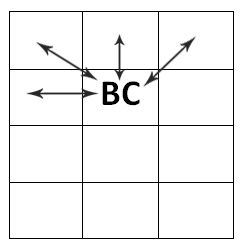
\includegraphics[scale=0.75]{a_test_galpat.png}  
  \caption{Тестирующий алгоритм GALPAT}
  \label{fig:domain:tests:galpat}
\end{figure}

Сложность алгоритма составляет $ 4n^{2} $. Покрывающая способность теста достаточно высокая, все неисправности типа Afs, TFs, CFs и SAFs обнаруживаются и локализуются. Псевдокод теста приведён в листинге~\ref{lst:domain:tests:galpat}.

\begin{lstlisting}[style=fsharpstyle, mathescape,escapeinside={/*@}{@*/},caption={Псевдокод реализации алгоритма GALPAT}, label=lst:domain:tests:galpat]
function GALPAT =
 Write background 0;
 for i in 0 .. 1 do
  for BC in 0 .. N-1 do
   Complement BC;
   for OC in 0 .. N-1 and OC != BC do
    Read BC;
    Read OC
   end for
   Complement BC;
   Write background 1;
 end for
end
\end{lstlisting}

\subsubsection{Тестирующий алгоритм WALPAT}
\label{sub:domain:tests:walpat}
Алгоритм WALPAT (Walking Pattern) очень похож на тест GALPAT. Различие лишь в том, что базовая ячейка считывается после того, как все остальные ячейки были просканированы. Сложность составляет $ 2n^{2} $. Тест проиллюстрирован на рисунке~\ref{fig:domain:tests:walpat}.

\begin{figure}[ht]
\centering
  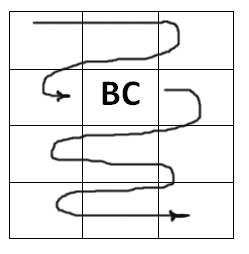
\includegraphics[scale=0.75]{a_test_walpat.png}  
  \caption{Тестирующий алгоритм WALPAT}
  \label{fig:domain:tests:walpat}
\end{figure}

Покрывающая способность данного теста, как и алгоритма Galloping Pattern, достаточно высокая, все неисправности типа Afs, TFs, CFs и SAFs обнаруживаются и локализуются. Псевдокод теста приведён в листинге~\ref{lst:domain:tests:walpat}.

\begin{lstlisting}[style=fsharpstyle, mathescape,escapeinside={/*@}{@*/},caption={Псевдокод реализации алгоритма WALPAT}, label=lst:domain:tests:walpat]
function WALPAT =
 Write background 0;
 for i in 0 .. 1 do
  for BC in 0 .. N-1 do
   Complement BC;
   for OC in 0 .. N-1 and OC != BC do
    Read OC
   end for
   Read BC;
   Complement BC;
   Write background 1;
 end for
end
\end{lstlisting}

\subsubsection{Тестирующий алгоритм Sliding}
\label{sub:domain:tests:sliding}
Тест основывается на алгоритме GALPAT, но вместо сдвига 1 по матрице ячеек, сдвигается целая диагональ(колонка, ряд) единиц. После каждого сдвига сканируется вся память. Тест представлен на рисунке~\ref{fig:domain:tests:sliding}.

\begin{figure}[ht]
\centering
  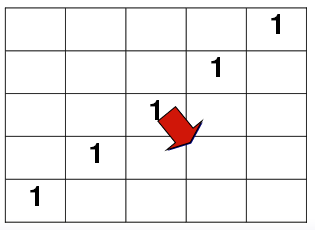
\includegraphics[scale=0.75]{a_test_sliding.png}  
  \caption{Тестирующий алгоритм Sliding}
  \label{fig:domain:tests:sliding}
\end{figure} 

Сложность алгоритма составляет $ 4n^{1.5} $. Покрывающая способность теста также довольно высокая, обнаруживаются все неисправности, за исключением некоторых неисправностей типа CFs.

\subsubsection{Тестирующий алгоритм Butterfly}
\label{sub:domain:tests:butterfly}
На протяжении теста базовая ячейка сдвигается по матрице памяти. При каждом сдвиге в цикле проверяются её ближайшие соседи в радиусе не более половины от длины строки и столбца матрицы ячеек. Тест представлен на рисунке~\ref{fig:domain:tests:butterfly}. 

\begin{figure}[ht]
\centering
  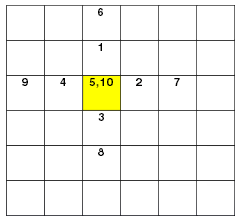
\includegraphics[scale=0.75]{a_test_butterfly.png}  
  \caption{Тестирующий алгоритм Butterfly}
  \label{fig:domain:tests:butterfly}
\end{figure} 

Сложность алгоритма составляет $ 5n \log n $. Тест обнаруживает все неисправности типа SAFs и некоторые из неисправностей типа AFs. Псевдокод теста приведён в листинге~\ref{lst:domain:tests:butterfly}.

\begin{lstlisting}[style=fsharpstyle, mathescape,escapeinside={/*@}{@*/},caption={Псевдокод реализации алгоритма Butterfly}, label=lst:domain:tests:butterfly]
function Butterfly =
 Write background 0;
 For i in 0 .. 1 do
  For BC in 0 .. N-1 do
   Complement BC;
   dist = 1; 
   While dist <= mdist do// mdist < 0.5 col/row length
    Read cell dist north from BC;
    Read cell dist east from BC;
    Read cell dist south from BC;
    Read cell dist west from BC;
    Read BC; 
    dist *=2;
   end while
   Complement BC
  end for
  Write background 1
 end for
end
\end{lstlisting}

\subsubsection{Тестирующий алгоритм Surround Disturb}
\label{sub:domain:tests:sd}
Алгоритм SD (Surround Disturb) Позволяет проверить поведение ячеек в строке, когда комплиментарные значения записываются в ячейки, расположенные на соседних рядах матрицы. Этот алгоритм разработан на предположении, что ячейки памяти наиболее чувствительны к помехам от своих ближайших соседей. Тест представлен на рисунке~\ref{fig:domain:tests:sd}. 

\begin{figure}[ht]
\centering
  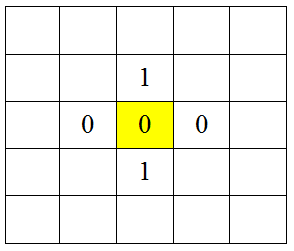
\includegraphics[scale=0.75]{a_test_sd.png}  
  \caption{Тестирующий алгоритм Surround Disturb}
  \label{fig:domain:tests:sd}
\end{figure} 

Псевдокод алгоритма представлен в листинге~\ref{lst:domain:tests:sd}.

\begin{lstlisting}[style=fsharpstyle, mathescape,escapeinside={/*@}{@*/},caption={Псевдокод реализации алгоритма Surround Disturb}, label=lst:domain:tests:sd]
For each cell [p,q] // row = p, col = q
{
 write 0 in cell[p,q-1];
 write 0 in cell[p,q];
 write 0 in cell [p, q+1];
 write 1 in cell[p-1,q];
 read 0 from cell[p,q+1];
 write 1 in cell[p+1,q];
 read 0 from cell[p, q-1];
 read 0 from cell[p,q];
}
\end{lstlisting}

\subsubsection{Маршевые тесты}
\label{sub:domain:tests:march}
Маршевые тесты являются самыми простыми и оптимальными для тестирования памяти. Они имеют линейную сложность и симметрию.
Маршевый тест состоит из конечной последовательности маршевых элементов. В свою очередь маршевый элемент состоит из последовательности операций чтения и записи, которые применяются ко всем ячейкам памяти в возрастающем или убывающем порядке адресов.
Все операции маршевого элемента выполняются до перехода к следующей ячейке памяти.
Обозначается маршевый элемент следующим образом: $rx$ - чтение из ячейки памяти, в которой должно храниться значение $x$; $wx$ - запись в ячейку памяти значения $x$; $\Uparrow$ - возрастающий порядок адресов (от 0 до n-1); $\Downarrow$ - убывающий порядок адресов (от n-1 до 0); $\Updownarrow$ - возрастающий или убывающий порядок адресов (направление не важно). 

Пример маршевого теста: $\{\Uparrow (w1); \Uparrow (r1,w0)\}$. Такой маршевый тест предполагает следующий алгоритм:

\begin{enumerate}
\item проходя от 0 до n-1 ячейки памяти записать 1 в i-ую ячейку;
\item проходя от 0 до n-1 ячейки памяти прочитать значение из i-ой ячейки, в которой должна быть 1, и записать в эту ячейку 0.
\end{enumerate}

В таблице~\ref{table:domain:tests:march_tests} представлены некоторые маршевые тесты.

\begin{table}[ht]
  \caption{Маршевые тесты}
  \label{table:domain:tests:march_tests}
  \begin{tabular}{| >{\centering}m{0.2\textwidth}
                  | >{\centering\arraybackslash}m{0.7\textwidth}|}
   \hline 
  {Наименование} & {Алгоритм} \\ \hline
   MATS & $\{\Updownarrow (w0); \Updownarrow (r0,w1); \Updownarrow (r1)\}$ \\ \hline
   MATS+ & $\{\Updownarrow (w0); \Uparrow (r0,w1); \Downarrow (r1,w0)\}$ \\ \hline
   MATS++ & $\{\Updownarrow (w0); \Uparrow (r0,w1); \Downarrow (r1,w0,r0)\}$ \\ \hline
   March X & $\{\Updownarrow (w0); \Uparrow (r0,w1); \Downarrow (r1,w0); \Updownarrow (r0)\}$ \\ \hline
   March C- & $\{\Updownarrow (w0); \Uparrow (r0,w1); \Uparrow (r1,w0); \Downarrow (r0,w1); \Downarrow (r1,w0); \Updownarrow (r0)\}$ \\ \hline
   March A & $\{\Updownarrow (w0); \Uparrow(r0,w1,w0,w1); \Uparrow (r1,w0,w1); \Downarrow (r1,w0,w1,w0); \Downarrow (r0,w1,w0)\}$ \\ \hline
   March B & $\{\Updownarrow (w0); \Uparrow(r0,w1,r1,w0,r0,w1); \Uparrow (r1,w0,w1); \Downarrow (r1,w0,w1,w0); \Downarrow (r0,w1,w0)\}$ \\ \hline
  \end{tabular}
\end{table}

Важным этапом в эволюции функциональных тестов ОЗУ стало применение неразрушающих методов тестирования. Необходимость в их использовании обусловлена критичностью современных приложений (сетевые серверы, системы управления) к показателям надежности \cite{March_Tests_Ivaniuk}. В таких случаях необходимо использовать тестовые алгоритмы, которые не разрушали бы содержимое ОЗУ. Преобразовать разрушающий маршевый тест в его неразрушающий аналог достаточно просто. Неразрушающие тесты имеют ряд обязательных требований: любой маршевый элемент начинается операцией чтения, отсутствует начальная инициализация памяти ($\Updownarrow (wx)$). После выполнения теста необходимо вернуть память в её первоначальное состояние. Идея неразрушающих тестов состоит в замене операций чтения и записи конкретных значений на операции чтения и записи прямых и обратных (комплиментарных) значений, хранящихся в ячейках памяти. 
Теперь неразрушающие операции маршевых тестов примут следующий вид: wdc, wd - запись dc и d значений в ячейку памяти; rdc, rd - чтение из ячейки памяти ожидаемых значений dc и d. Значение dc есть комплиментарное значение к d. На примере теста MATS+ его неразрушающий аналог будет выглядеть следующим образом: $\{\Uparrow (rd,wdc); \Downarrow (rdc,wd)\}$.

\subsection{Обзор существующих аналогов}
\label{sub:domain:analogue}
В открытых источниках информация о существующих аналогах не найдена. Даже если таковые имеются, то они скорее всего являются закрытыми инструментами компаний, занимающихся проблемой тестирования памяти. Вследствие этого факта сравнение с ними невозможно. Исходя из отсутствия свободно распространяемых утилит по верификации тестирующих алгоритмов оперативных запоминающих устройств, разработка данного программного средства имеет смысл.

\subsection{Постановка задачи}
\label{sub:domain:task}
В результате выполнения дипломного проекта должна быть разработана библиотека, написанная на языке С++, для верификации тестирующих алгоритмов оперативных запоминающих устройств со следующими спецификациями:
\begin{itemize}
  \item разрабатываемое ПО должно иметь возможность запускаться под платформами Windows(7,8,10);
  \item разрабатываемое ПО должно позволять производить верификацию тестирующих алгоритмов ОЗУ, в зависимости от требований
конечного пользователя;
  \item подвергаться тестированию должна динамическая память, симулируемая инструментом DRAMSim2;
  \item время работы ПО должно быть приемлемым.
\end{itemize}




